\documentclass{beamer}
\usepackage{graphicx}
\usepackage{amsmath,amssymb,amsfonts}
\usepackage{wrapfig}
\usepackage[utf8]{inputenc}
\usepackage{listings}
\lstset{
  basicstyle=\ttfamily\footnotesize,
  showspaces=false,
  stringstyle=\color{orange},
  %frame=single,
  showstringspaces=false,
  xleftmargin=1cm,
  keywordstyle=\bfseries,
  commentstyle=\itshape\color{Gray}
}
\renewcommand{\ttdefault}{pcr}

\usecolortheme{crane}
%$\setbeamercovered{dynamic}
\setbeamertemplate{items}[circle]
\setbeamertemplate{blocks}[rounded][shadow=false]
\setbeamertemplate{navigation symbols}{}
\setbeamertemplate{footline}[frame number]{}

\title{Algorithmic Analysis\\ of Code-Breaking Games}
\author{\textbf{Miroslav Klimoš} \\\medskip Advisor: prof. RNDr. Antonín Kučera Ph.D.}

\date{June 2014}

\begin{document}

\begin{frame}[plain]
\begin{center}

\includegraphics[width=20mm]{logo_fi.pdf}
\end{center}
\vspace{-5mm}
\maketitle
\end{frame}

\begin{frame}{Code-breaking games}
\begin{itemize}\itemsep 10pt
\item 2 players: \textbf{codemaker + codebreaker}
\item codemakers selects a \textbf{secret code}
\item codebreaker strives to reveal the code through \textbf{experiments}
\item for each experiment, codemaker releases some \\\textbf{partial information} about the code
\end{itemize}
\end{frame}

\begin{frame}{Mastermind}
\begin{columns}
 \begin{column}{.35\textwidth}
 \centering
 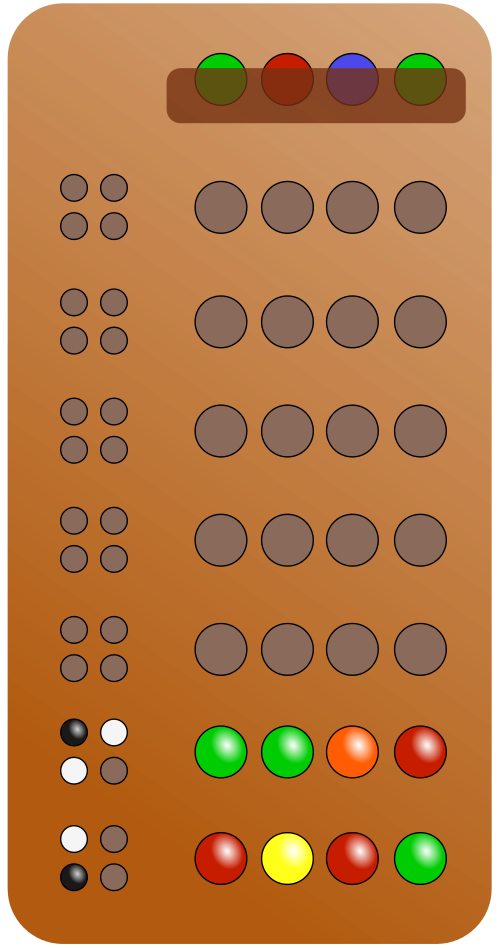
\includegraphics[width=3cm]{../pictures/mastermind.png}
 \end{column}

 \begin{column}{.6\textwidth}
  \begin{itemize}
  \item Code: 4 pegs $\times$ 6 colours
  \item Experiment $=$ guess
  % \item Evaluation with black and white markers\\
  \end{itemize}
  \begin{center}
  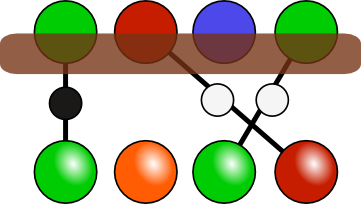
\includegraphics[width=3cm]{../pictures/mastermind-matching.png}
  \end{center}
 \end{column}
\end{columns}
\end{frame}

\begin{frame}{The counterfeit coin}
\begin{quote}
You are given 12 coins, all except one having the same weight.
It is not known whether the counterfeit coin is heavier or lighter.
Identify the counterfeit coin and its weight relative to the others
  in the minimal number of weighings.
\end{quote}
\end{frame}

\begin{frame}{Challenges}
\begin{enumerate}
\item Formal model of code-breaking games
\item Strategies for experiment selection
\item Method for symmetry detection
\item Algorithms for strategy evaluation and synthesis
\item Computer language for game specification
\item Implementation of proposed algorithms
\end{enumerate}
\end{frame}

\begin{frame}{Formal model}
\begin{itemize}
\item Game description
\begin{itemize}
\item set of propositional variables $X$
\item initial constraint $\varphi$
\item set of \textbf{experiments} $E$
\end{itemize}

\item Secret code: valuation of $X$ (satisfying $\varphi$)
\item Partial information: formula in $X$
\item Strategy (memory-less): function $\textsc{form}_X \rightarrow E$
\end{itemize}
\end{frame}

\begin{frame}{Example -- the counterfeit coin}
\begin{itemize}
\item variables $\{x_1, x_2, x_3, x_4, y\}$
\item initial constraint $\textsc{exactly}_1(x_1, x_2, x_3, x_4)$
\item experiment ``coin 1 $\times$ coin 2'' can result in \medskip
  \begin{enumerate}\itemsep 5pt
  \item[``$<$'':] $(x_1\wedge \neg y) \vee (x_2\wedge y)$
  \item[``$>$'':] $(x_1 \wedge y) \vee (x_2\wedge\neg y)$
  \item[``$=$'':] $\neg x_1 \wedge \neg x_2 $
  \end{enumerate}
\end{itemize}
\end{frame}

\begin{frame}{Strategies}

\begin{block}{Max-models strategy}
Select an experiment that minimizes the maximal number
  of possibilities for the code in the next round.
\end{block}

\bigskip
\begin{itemize}\itemsep 5pt
\item in Mastermind(4,6), this is worst-case optimal
\item Generalization: one-step look-ahead strategies
\end{itemize}

\end{frame}

\begin{frame}{Symmetry detection}
\begin{itemize}
\item Problem: symmetries enlarge the state space
\item Solution: experiment equivalence
\end{itemize}
\pause
\centerline{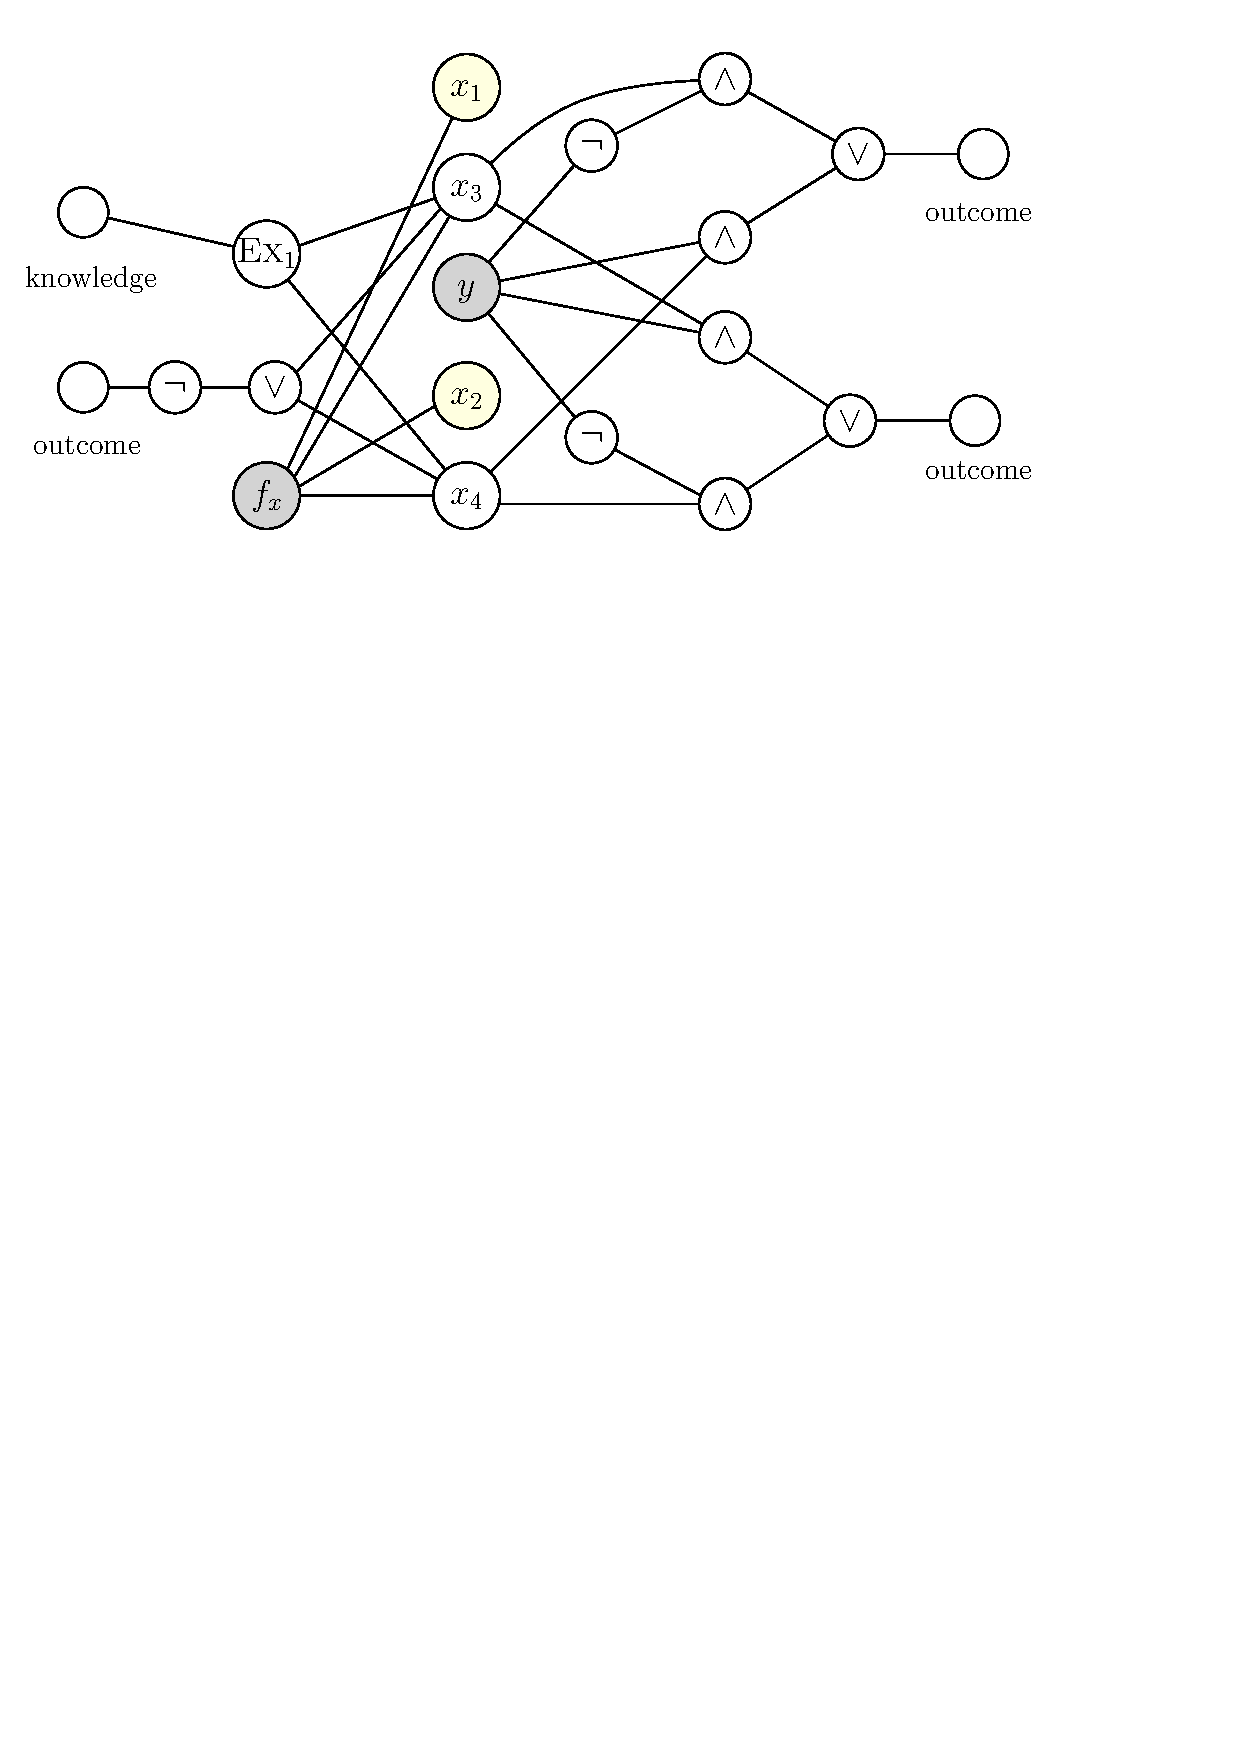
\includegraphics[width=7cm]{../pictures/exp-graph-sim.pdf}}
\begin{itemize}
\item Reduction to isomorphism of labelled graphs
\item Tools available for graph canonization (Bliss)
\end{itemize}
\end{frame}

\begin{frame}{Algorithmic problems}
\begin{block}{Strategy analysis}
Compute the average-case/worst-case number of experiments needed
  to reveal the code by a given strategy.
\end{block}\pause
\bigskip
\begin{block}{Optimal strategy synthesis}
Synthesise the average-case/worst-case optimal strategy.
\end{block}\pause

\bigskip
\centerline{$\Longrightarrow$ intelligent backtracking}
\end{frame}

\begin{frame}[fragile]{Game specification language}
\begin{itemize}
\item Based on the formal model
\item Python preprocessing for easier generation
\end{itemize}

% # Helper function for generating strings that represent range of parameters
% # For example, params(2,5) = "X$2, X$3, X$4, X$5"
% params = lambda n0, n1: "|".join("X$" + str(i) for i in range(n0, n1+1))
\pause
\begin{lstlisting}[language=Python]
n = 4
xvars = ["x1", "x2", "x3", "x4"]
VARIABLES(xvars + ["y"])
CONSTRAINT("Exactly-1(%s)" % ",".join(xvars))
ALPHABET(xvars)
MAPPING("X", xvars)

for m in range(1, n//2 + 1):
  EXPERIMENT("weighing" + str(m), 2*m)
  PARAMS_DISTINCT(range(1, 2*m + 1))
  OUTCOME("lighter", "((%s) & !y) | ((%s) & y)" ...
  OUTCOME("heavier", "((%s) & y) | ((%s) & !y)" ...
  OUTCOME("same", "!(%s)" % params(1, 2*m))
\end{lstlisting}
\end{frame}

\begin{frame}{Implementation -- the Cobra tool}
\begin{itemize} \itemsep 10pt
\item Command-line tool written in C++
\item Modes of operation
  \begin{itemize}
  \item Overview
  \item Simulation
  \item Strategy analysis
  \item Optimal strategy synthesis
  \end{itemize}
\item Uses SAT solvers (Minisat, Picosat)
\item Uses graph canonization tool (Bliss)
\end{itemize}
\end{frame}

\begin{frame}{Conclusions}
\begin{itemize}
\item Challenges
\begin{enumerate}[\checkmark]
\item Formal model based on propositional logic
\item Strategies for experiment selection
\item Symmetry detection based on graph isomorphism
\item Algorithms for strategy evaluation and synthesis
\item Computer language built on top of Python
\item Implementation in the Cobra tool
\end{enumerate}\bigskip\pause
\item Applications
\begin{itemize}
\item easily reproduce existing results
\item evaluate new strategies
\item analyse other code-breaking games
\end{itemize}
\end{itemize}
\end{frame}

\end{document}


